\documentclass[aspectratio=169]{beamer}
\usepackage{color,amsmath}
\usepackage{subfigure}
\usepackage{booktabs}
\usepackage{framed}
\usepackage{comment}
\usepackage{url}


%%%%%%%%%%%%%%%%%%%%%%%%%%
\title[]{Introduction to group activity}
\author[]{Matthew J. Salganik\\Department of Sociology\\Princeton University}
\date[]{Summer Institute in Computational Social Science\\June 21, 2018
\vfill
\begin{flushleft}
{\scriptsize
The Summer Institute in Computational Social Science is supported by grants from the Russell Sage Foundation and the Alfred P. Sloan Foundation.}
\end{flushleft}
\begin{flushright}

\includegraphics[width=0.1\textwidth]{figures/cc-by.png}
\end{flushright}
}
\begin{document}
%%%%%%%%%%%%%%%%%%%%%%%%%%
\frame{\titlepage}
%%%%%%%%%%%%%%%%%%%%%%%%%%
\begin{frame}

\begin{center}
\only<1>{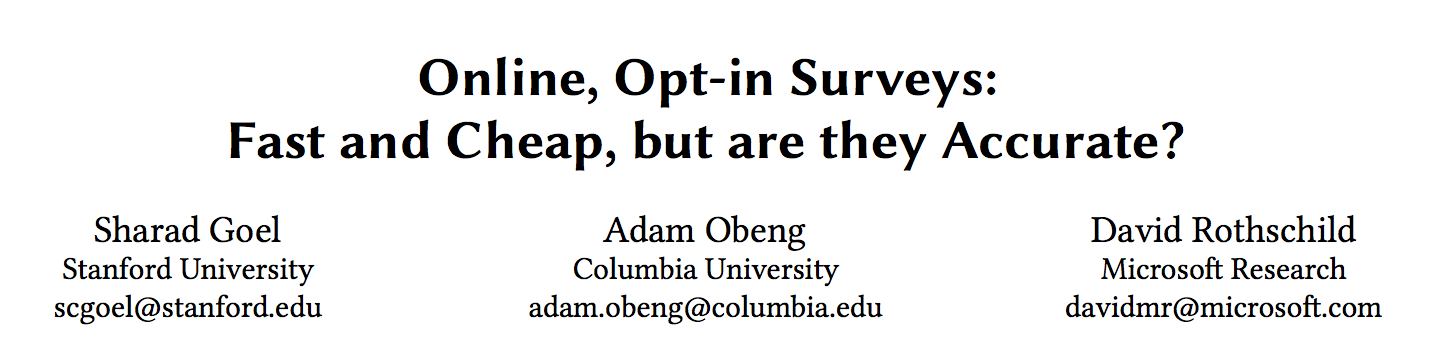
\includegraphics[width=0.9\textwidth]{figures/goel_online_2017_title}}
\only<2>{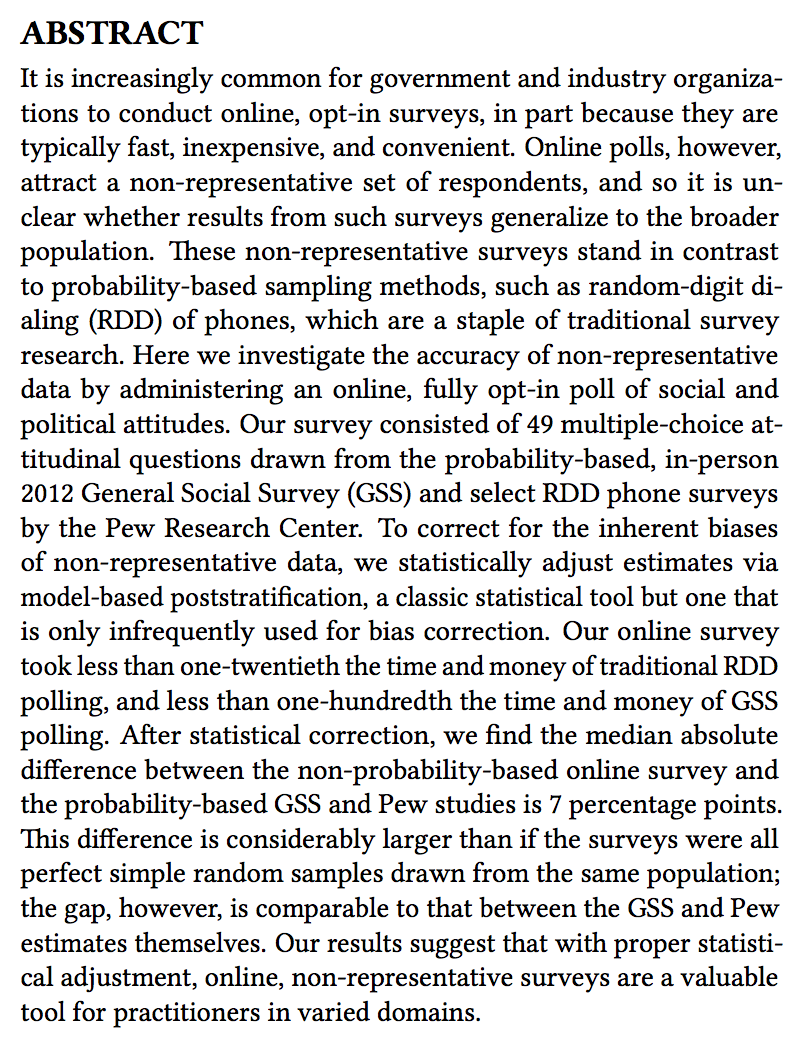
\includegraphics[width=0.4\textwidth]{figures/goel_online_2017_abstract}}
\end{center}

\vfill
\url{https://5harad.com/papers/dirtysurveys.pdf}

\end{frame}
%%%%%%%%%%%%%%%%%%%%%%%%%%%
\begin{frame}

Activity:
\begin{itemize}
\item Design a questionaire using questions already asked on high quality surveys
\pause
\item Recruit participants from Amazon Mechanical Turk and have them complete your questionnaire  
\pause
\item Compare results from your survey to the results from the high-quality survey
\pause
\item Try different approaches to weighting and see how the change the estimates
\pause
\item De-identify and open-source data 
\end{itemize}

\end{frame}
%%%%%%%%%%%%%%%%%%%%%%%%%%
\begin{frame}

This activity will give you practice:
\begin{itemize}
\item Designing questionnaires
\pause
\item Collecting survey data
\pause
\item Analyzing survey data (data wrangling and post-stratification)
\pause
\item Working with Amazon Mechanical Turk
\pause
\item Archiving data for other researchers
\end{itemize}

\vfill
Remember: This is a learning activity so try whatever you want.

\end{frame}
%%%%%%%%%%%%%%%%%%%%%%%%%%%
\begin{frame}

Our recommended work flow:
\begin{itemize}
\item Create survey on Google Forms (we have a template)
\item Deploy to MTurk
\item Take a break
\end{itemize}

\end{frame}
%%%%%%%%%%%%%%%%%%%%%%%%%%
\begin{frame}

\begin{center}
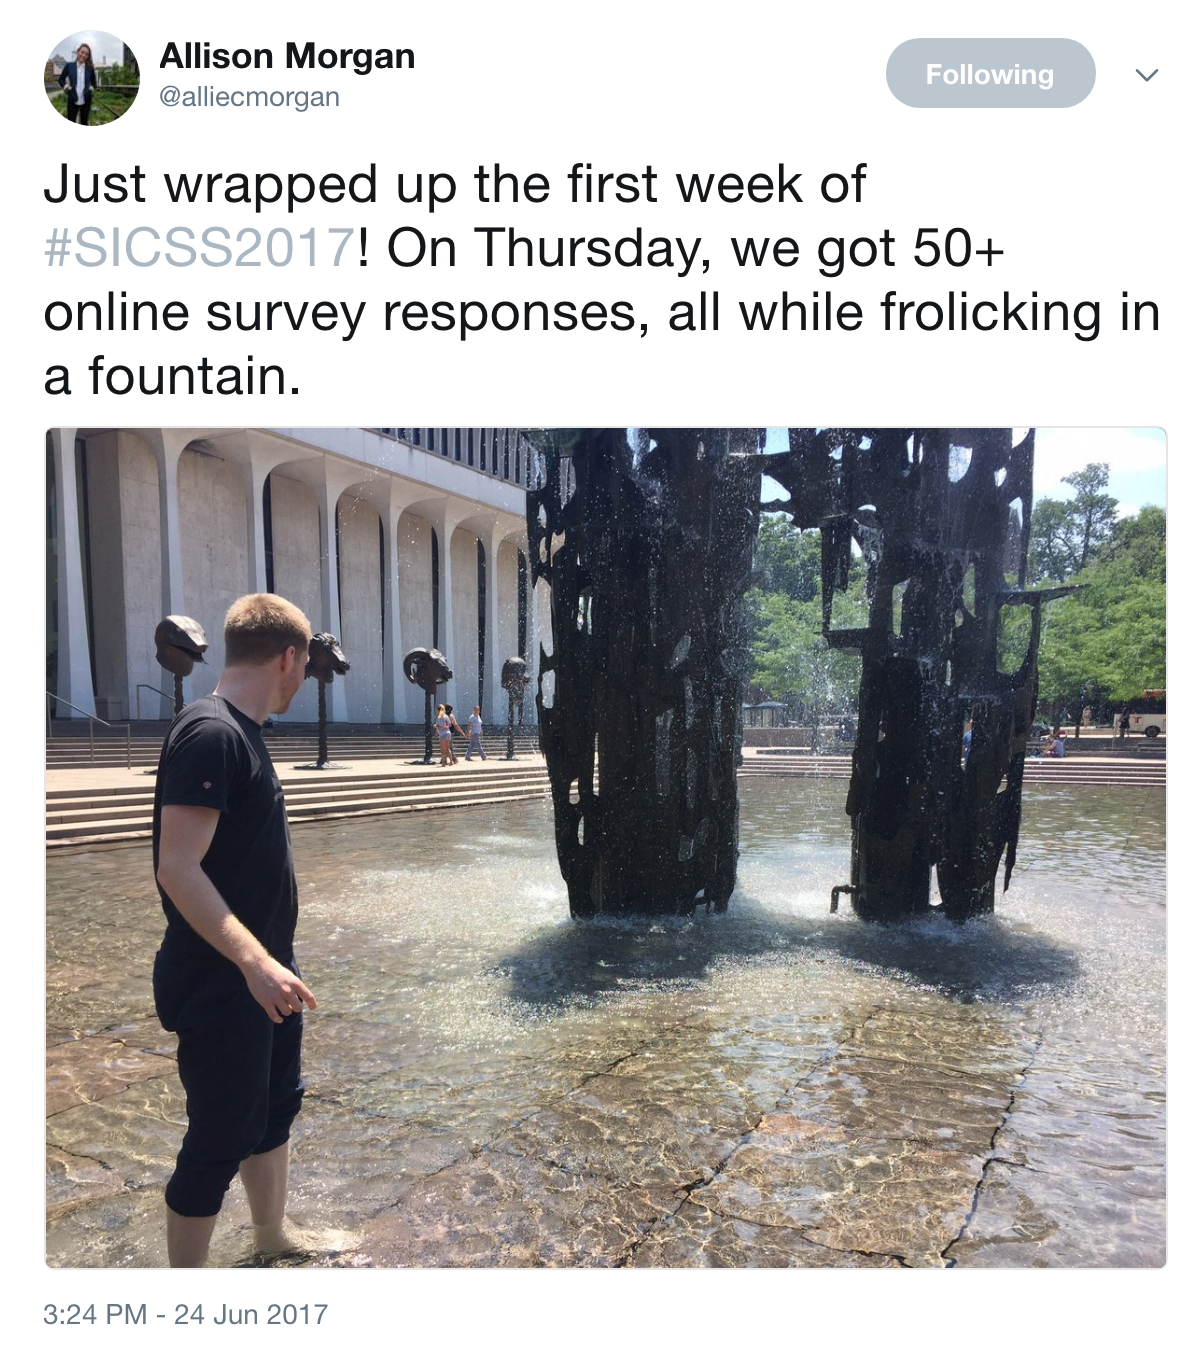
\includegraphics[width=0.4\textwidth]{figures/morgan_tweet}
\end{center}

\end{frame}
%%%%%%%%%%%%%%%%%%%%%%%%%%
\begin{frame}

Our recommended work flow:
\begin{itemize}
\item Create survey on Google Forms
\item Deploy to MTurk
\item Take a break
\item Validate and pay workers
\item Analyze the much larger sample that we have collected for you
\end{itemize}

\end{frame}
%%%%%%%%%%%%%%%%%%%%%%%%%%
\begin{frame}

A quick and dirty tour of the post-stratification methods we will use

\end{frame}
%%%%%%%%%%%%%%%%%%%%%%%%
\begin{frame}
\frametitle{Cell-based Poststratification}

Let's split the sample into $H$ mutually exclusive and exhaustive groups.  

\begin{equation*}
\hat{\bar{y}}_{post} = \sum_{h=1}^H \frac{N_h}{N} \hat{\bar{y}}_h
\end{equation*}
where 
\begin{itemize}
\item $N$: size of the population
\item $N_h$: size of group $h$
\item $\hat{\bar{y}}_h$: estimated average outcome for group $h$
\end{itemize}
\vfill
Roughly, we are producing estimates for each group and then putting them together in the right way.

\end{frame}

\begin{frame}
\frametitle{Cell-based Poststratification}

Assumptions:
\begin{itemize}
\item The realized sample $s$ is partitioned into $H$ groups, $s_1, s_2, \ldots s_H$
\item Given $s$, all elements in $s_k$ are assumed to have the same response probability; different groups can have different response probabilities
\item Equivalent to data is missing completely at random (MCAR) within each group
\item ``Response Homogeneity Group Model'' (RHG Model), see Sarndal et al.\ (1992) Sec 15.6.2 (``A Useful Response Model'')
\end{itemize}

\vfill
If RHG model holds (and some other minor technical conditions), then the poststratification estimator is unbiased.  See Sarndal et al.\ (1992) Result 15.6.1 

\end{frame}

\begin{frame}
\frametitle{Bias of cell-based poststratification estimator from non-response}

If RHG does not hold and if the original sample is simple random sampling without replacement, then (Bethlehem, Cobben, and Schouten 2011, sec. 8.2.1):

$$bias(\hat{\bar{y}}_{post}) = \frac{1}{N} \sum_{h=1}^H \frac{cor(\phi_i, y_i)^{(h)} S(\phi_i)^{(h)} S(y_i)^{(h)}}{\bar{\phi}^{(h)}}$$

So, how should we create the $H$ groups? \pause
\begin{itemize}
\item form homogeneous groups where there is little variation in response propensity $(S(\phi_i)^{(h)} \approx 0)$ and the outcome $(S(y_i)^{(h)} \approx 0)$ \pause
\item form groups where the people that you see are like the people that you don't see $(cor(\phi_i, y_i)^{(h)} \approx 0)$
\end{itemize}

\vfill
In practice this can be difficult because you want to form many groups, but then you have noisy estimates for each group.

\end{frame}

\begin{frame}

\begin{equation*}
\hat{\bar{y}}_{post} = \sum_{h=1}^H \frac{N_h}{N} \hat{\bar{y}}_h
\end{equation*}
where 
\begin{itemize}
\item $N$: size of the population
\item $N_h$: size of group $h$
\item $\hat{\bar{y}}_h$: estimated average outcome for group $h$
\end{itemize}
\vfill

Use this estimator in three steps:
\begin{enumerate}
\item Chop up the sample into groups \pause
\item Estimate the mean in each group \pause
\item Combine the estimates for each group into an overall estimate
\end{enumerate}

\end{frame}

\begin{frame}

Note:
\begin{itemize}
\item Horvitz-Thompson estimation is individual-based weight
\item Poststratification can better be understood as a group-based weight
\end{itemize}

\end{frame}

\begin{frame}

Three increasingly sophisticated ways to make group estimate $\hat{\bar{y}}_h$
\begin{itemize}
\item cell-based poststratification
\item model-based poststratification
\item multilevel regression postratification (Mr. P)
\end{itemize}

\end{frame}


\begin{frame}{Data}

\begin{itemize}
\item Our survey data comes from a survey of 684 people on MTurk collected in less than a week ago
\item We will compare to high-quality telephone surveys from the Pew Research Center
\item To poststratify our survey data, we will use data from the Census Bureau about the population of the US
\end{itemize}

\end{frame}

\begin{frame}{Data}

Example questions (after question wrangling):
\begin{itemize}
\item If you were making up the budget for the federal government this year would you increase funding for scientific research?\pause
\item Do you not smoke cigarettes at all? \pause
\item All in all, are you satisfied with the way that things are going in this country today? \pause
\end{itemize}

\vfill
We use multiple questions because estimates are also a property of a question not just a sample.

\end{frame}

\begin{frame}{Simple cell-based poststratification}

Let's do lots of groups.
\begin{itemize}
\item gender (2 groups)
\item age (4 groups)
\item race (5 groups)
\item region (4 groups)
\item Makes 160 $(2 \times 4 \times 5 \times 4)$ groups
\end{itemize}

\end{frame}

\begin{frame}{Simple cell-based poststratification}

\begin{equation*}
\hat{\bar{y}}_h = \frac{\sum_{i \in h} y_i}{n_h}
\end{equation*}

\vfill
$h$ is a group described by a unique combination of gender (2 groups) $\times$ age (4 groups) $\times$ race (5 groups) $\times$ region (4 groups) 

\end{frame}

\begin{frame}{Cell-based poststratification}

\begin{center}

\includegraphics[width=0.5\textwidth]{figures/fail}
\end{center}

\vfill

\begin{itemize}
\item We can't make an estimate for each group.  For example, we don't have any female, 65+, Hispanic living in the South. \pause
\item This problem can arise if you have too many cell.  We have a crude work-around in the code we provide. 
\end{itemize}

\end{frame}

\begin{frame}{Model-based poststratification}

\begin{equation*}
\hat{\bar{y}}_{post} = \sum_{h=1}^H \frac{N_h}{N} \hat{\bar{y}}_h
\end{equation*}
where
$\hat{\bar{y}}_h$ comes from

\begin{align*}
Pr(y_i = 1) = logit^{-1} (\beta_0 + \\
 \beta_{male} \cdot male_i+ \\
 \beta_{30-49} \cdot 30-49_i + \beta_{50 - 64} \cdot 50-64_i+ \beta_{65+} \cdot 65_i +\\
 \beta_{afr-am} \cdot afam_i + \beta_{as-am} \cdot asam_i+ \beta_{hispanic} \cdot hisp_i + \beta_{other} \cdot other_i + \\
 \beta_{midwest} \cdot midwest_i + \beta_{south} \cdot south_i + \beta_{west} \cdot west_i)
\end{align*}

\end{frame}

\begin{frame}{Mr. P}

\begin{center}
\only<1>{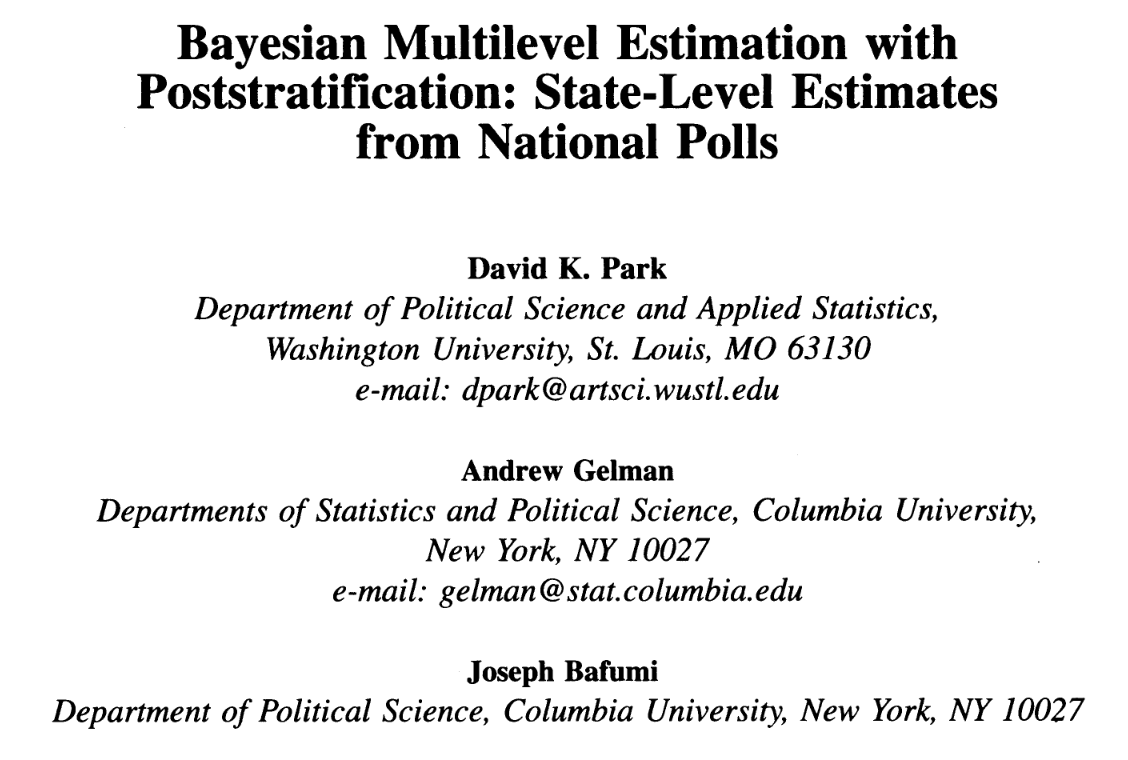
\includegraphics[width=0.8\textwidth]{figures/park_bayesian_2004_title}}
\only<2>{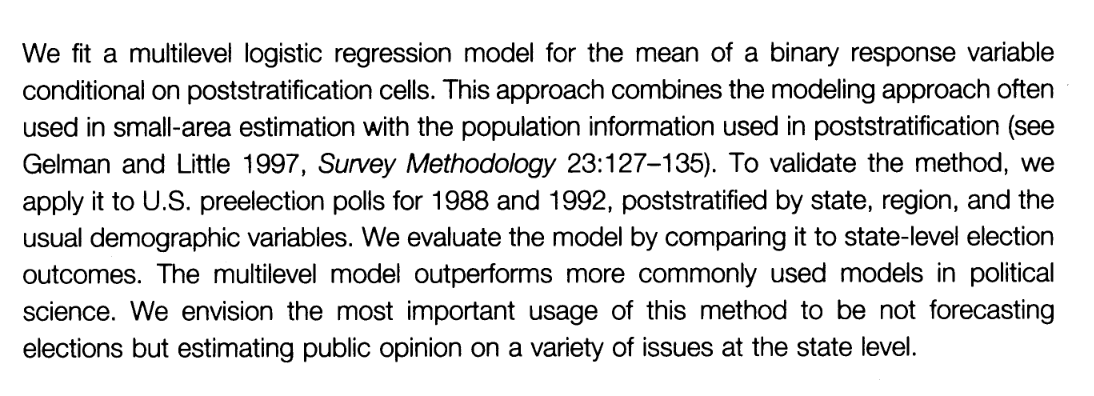
\includegraphics[width=\textwidth]{figures/park_bayesian_2004_abstract}}
\end{center}

\vfill
\url{https://www.jstor.org/stable/25791784} \\ See also Gelman and Hill (2007), Chapter 14 (``Multilevel logistic regression'')

\end{frame}

\begin{frame}{Mr. P.}

$\hat{\bar{y}}_h$ comes from\\

\begin{align*}
Pr(y_i = 1) = logit^{-1} (\beta_0 + \\
 \beta_{male} \cdot male_i + \\
 \alpha_{k[i]}^{age} + \\
 \alpha_{k[i]}^{race} + \\
 \alpha_{k[i]}^{region})
\end{align*}

\begin{align*}
\alpha_{k}^{age} \sim N(0, \sigma^2_{age}) \text{ for } k = 1, \ldots, 4 \\
\alpha_{k}^{race} \sim N(0, \sigma^2_{race}) \text{ for } k = 1, \ldots, 5 \\
\alpha_{k}^{region}  \sim N(0, \sigma^2_{region}) \text{ for } k = 1, \ldots, 4
\end{align*}

Priors determined by RStanarm (\url{https://cran.r-project.org/web/packages/rstanarm/vignettes/priors.html})

\end{frame}

% Talk about two models fighting, shrinking coefficients toward 0

\begin{frame}{Notes}

\begin{itemize}
\item Modeling allows you to make more estimates for smaller groups \pause
\item These techniques is widely used by modern pollsters (e.g., YouGov) and political scientists \pause
\item These same techniques can be for small-area estimation 
\end{itemize}

\end{frame}

\begin{frame}{To learn more about Mr. P.}

{\footnotesize
Generally optimistic:
\begin{itemize}
\item Park, Gelman, and Bafumi. 2004. ``\textcolor{blue}{\href{https://www.jstor.org/stable/25791784}{Bayesian Multilevel Estimation with Poststratification: State-Level Estimates from National Polls}}.'' \textit{Political Analysis}.
\item Lax and Phillips. 2009. ``\textcolor{blue}{\href{https://www.jstor.org/stable/25193870}{How should we estimate public opinion in the states?}}'' \textit{American Journal of Political Science}.
\item Ghitza and Gelman. 2013. ``\textcolor{blue}{\href{https://www.jstor.org/stable/23496652}{Deep Interactions with MRP: Election Turnout and Voting Patterns Among Small Electoral Subgroups}}.'' \textit{American Journal of Political Science}.
\item Warshaw and Rodden. 2012. ``\textcolor{blue}{\href{http://www.jstor.org/stable/10.1017/s0022381611001204}{How should we measure district-level public opinion on individual issues?}}'' \textit{Journal of Politics}.
\item Downs et al. 2018. ``\textcolor{blue}{\href{https://doi.org/10.1093/aje/kwy070}{Multilevel Regression and Poststratification: A Modelling Approach to Estimating Population Quantities From Highly Selected Survey Samples}}.'' \textit{American Journal of Epidemiology}.
\end{itemize}
Generally cautious:
\begin{itemize}
\item Buttice and Highton. 2013. ``\textcolor{blue}{\href{http://www.jstor.org/stable/24572674}{How Does Multilevel Regression and Poststratification Perform with Conventional National Surveys?}}'' \textit{Political Analysis}.
\end{itemize}
}

\end{frame}
%%%%%%%%%%%%%%%%%%%%%%%%%%
\begin{frame}

Our recommended work flow:
\begin{itemize}
\item Create survey on Google Forms
\item Deploy to MTurk
\item Take a break
\item Validate and pay workers
\item Analyze the much larger sample that we have collected for you
\item De-identify and open-source the data that you collected
\end{itemize}

\end{frame}
%%%%%%%%%%%%%%%%%%%%%%%%%%

\end{document}
